\subsection{Habermas: Kommunikatives Handeln}

\epigraph{
		``Reading understanding is the inherent telos of human speech.''}
	{
		\emph{Jürgen Habermas
	}

Dass Schule und Demokratie eng mit Kooperation und Kommunikation verbunden ist, wird bereits anhand von beispielsweise \citeauthor{Kleinberg-2009-oz} und \citeauthor{mead-1934en} deutlich.
Die Intersubjektivität ist bei beiden gegeben:
Nach Meads symbolischem Interaktionismus entsteht die Identität schließlich immer im Kontakt mit anderen Individuen und Kleinbergs Kooperationslose Spiele enden nicht notwendigerweise im sozialen Optimum.

Jürgen Habermas \citeauthor{Habermas-1998-aa} postuliert nun in seinem 1998 erschienen Text "On the Pragmatics of Communication" einen Telos menschlichen Handelns und menschlicher Sprache und unterscheidet zwischen verschiedenen Handlungsformen \autoref{fig:handlungsformen} (\autopageref{fig:handlungsformen}).

\begin{figure}[htbp]
	\begin{center}
	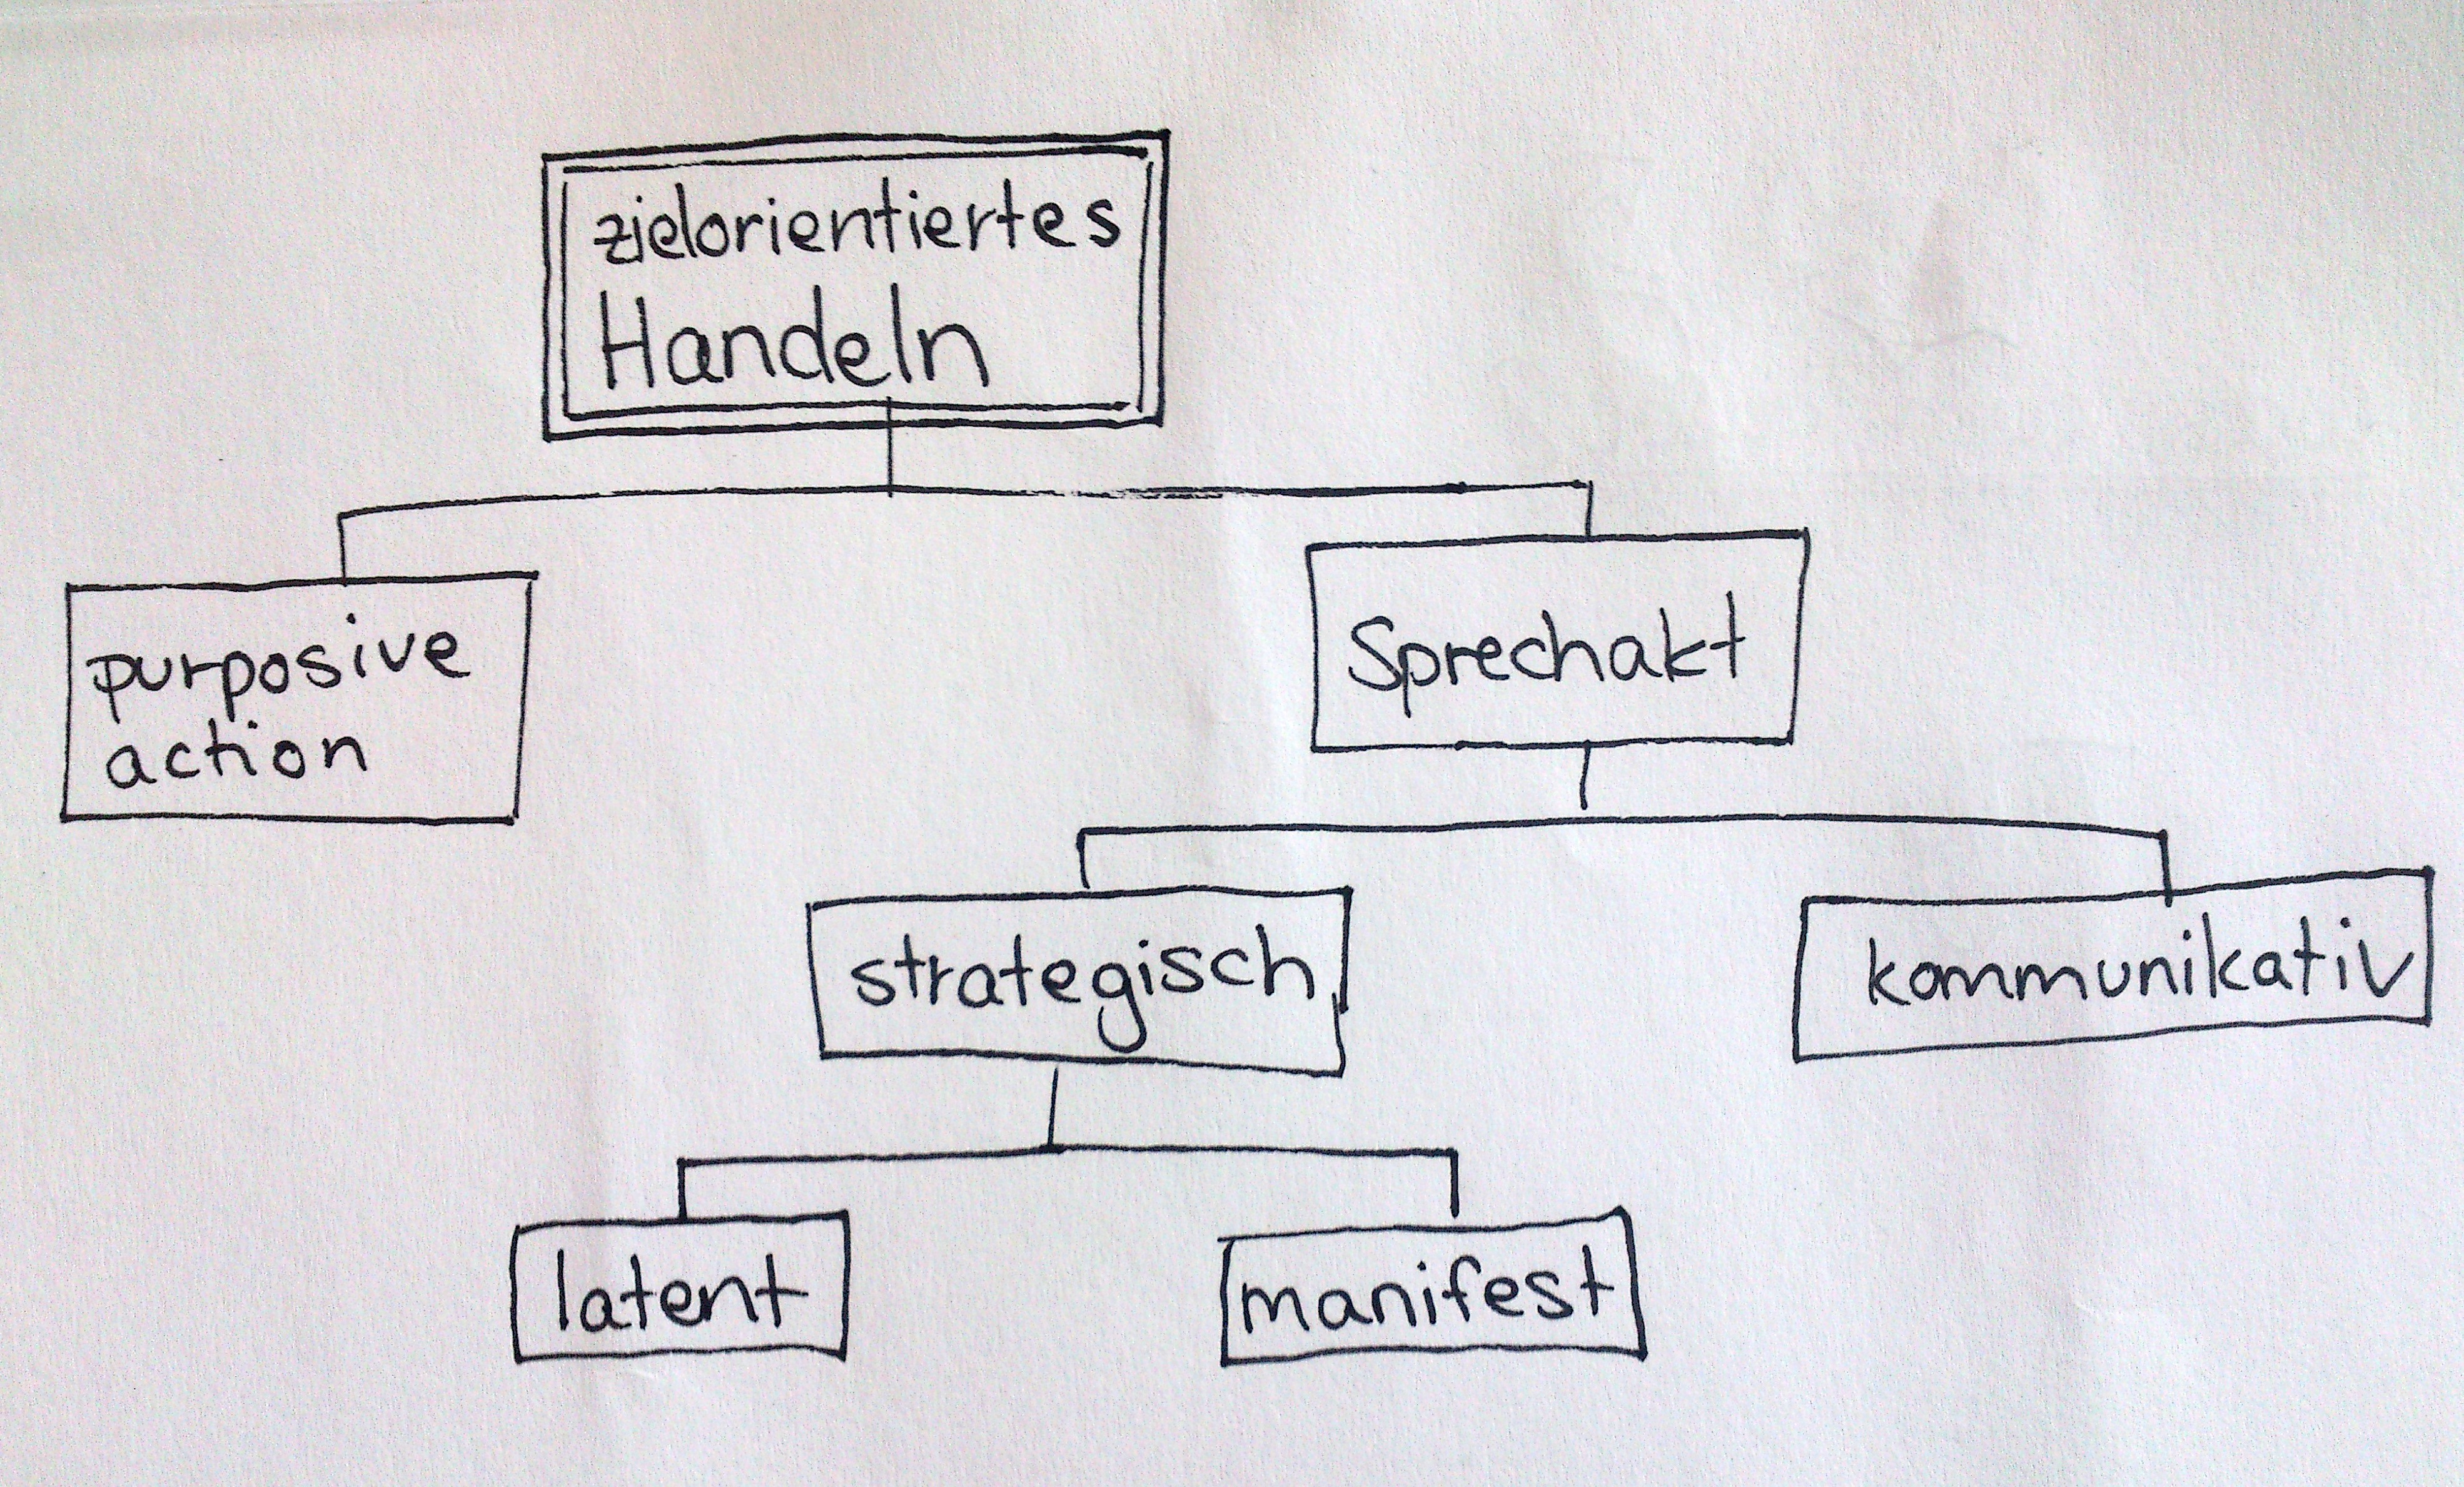
\includegraphics[width=1\textwidth]{img/Habermas_Baumuebersicht.jpg}
	\caption{Handlungsformen nach \cite{Habermas-1998-aa}}
	\label{fig:handlungsformen}
	\end{center}
\end{figure}

Dabei differenziert er zunächst zwischen Handlungen an Objekten in der fassbaren Realität und Handlungen in der sozialen Welt, also Sprechakten, die sich insbesondere in ihren Zielen unterscheiden.

Während die Ziele der Handlungen am Objekt laut \citeauthor{Habermas-1998-aa} kausal herbeigeführt werden können und die Mittel unabhängig vom Zweck stehen, können die Ziele eines Sprechaktes nicht unter diesen Kategorien zusammengefasst werden.
Denn der Sprechakt enthält, im Gegensatz zum Handeln am Objekt, ein sogenanntes illokutives Element, das dem Gesprächsparter die dem Sprechakt zugrundeliegende Absicht des Handelnden offenbart.
Einmal ist deshalb die Annahme der Kausalität unmöglich, denn das Ziel der Verständigung erfordert die Kooperation mit einer zweiten Person und kann damit nicht den selben innerweltlichen Status haben, wie eine Handlung am Objekt.
Außerdem ist auch die Trennung von Mittel und Zweck in der Sprache nicht möglich:

	\begin{quote}
		``the medium of natural language and the telos of reaching understanding interpret one another reciprocally, one cannot be explained without recourse to the other.''
			\citep[218]{Habermas-1998-aa}
	\end{quote}

Wenn Hanna, Assistentin der Akademieleitung, im Plenum beispielsweise darauf hinweist, dass die Hilfe beim Drucken der Akademie-T-Shirt wichtig für das Gelingen des Projekts ist, muss Sie, um eben diese Verständigung zu erreichen auf Sprache zurück greifen, welche wiederrum einen Verständigungs-Telos impliziert.
Führen wir diesen Gedanken weiter geraten wir schnell in einen Kreislauf, der die Rekursivität zwischen Sprache und dem Ziel der Verständigung deutlich macht.

Das Telos der illokutiven Verständigung als universelles Ziel menschlicher Sprache steht für \citeauthor{Habermas-1998-aa} teleologisch fest und ist der Ausgangspunkt seiner an die des amerikanischen Philosophen John Rogers Searle und seines britischen Kollegen John Langshaw Austin angelehnten Sprechakttheorie.

Grundsätzlich geht \citeauthor{Habermas-1998-aa}, wie Searle und Austin, davon aus, dass mit jedem Sprechakt automatisch ein Gültigkeitsanspruch auf das Gesagte erhoben wird.
Er grenzt sich allerdings von deren Vorstellung ab, die von Sprechakten aufgestellten Gültigkeitsansprüche würden nur aus Aussagenlogik bestehen.
Er sieht diese stattdessen nur als einen Teil der Gültigkeitsansprüche, die an Sprechakte gestellt werden müssen.

Sagt Mihai, Assistent der Akademieleitung, beispielsweise ``Wir sollten dem Küchenpersonal etwas vorsingen, weil es jeden Tag unser Essen zubereitet'' kann nach \citeauthor{Habermas-1998-aa} zwar sowohl auf die objektive Wahrheit (Bereitet das Küchenpersonal wirklich unser Essen zu?) aber eben auch auf die normative Richtigkeit (Ist Vorsingen eine angemessene Dankesgeste), die subjektive Authenzithät (Ist das Gesagte auch so gemeint oder wird Mihai von Kerstin gezwungen diesen Vorschlag zu machen?) und die sprachliche Verständlichkeit überprüft werden.
Für \citeauthor{Habermas-1998-aa} muss jeder einzelne dieser Gültigkeitsansprüche anfechtbar sein um kommunikatives Handeln zu ermöglichen.

Generell differenziert er zwischen strategischem und kommunikativem Handeln, wobei er letzteres für erstrebenswerter hält.
Zwar steht für \citeauthor{Habermas-1998-aa} grundsätzlich hinter jeder Handlung ein ``action plan'', also ein Ziel, allerdings geht er auch davon aus, dass für eine erfolgreiche Kommunikation die Beilegung dieses ``action plans'' nötig ist, um ausschließlich illokutive Ziele zu verfolgen.
Wird dies nicht getan, spricht \citeauthor{Habermas-1998-aa} von strategischem Handeln, welches perlokutive Ziele, in den Vordergrund stellt, also eine bestimmte Wirkung beim Gegenüber erreichen möchte.
Dabei gibt es wiederum zwei Arten von strategischem Handeln:
Latent strategisches Handeln und manifest strategisches Handeln.

Das \emph{latent strategische Handeln} zeichnet sich dadurch aus, dass der Sprechende zwar vorgibt illokutive Ziele zu verfolgen und einen anzweifelbaren Gültigkeitsanspruch aufzustellen, in Wirklichkeit aber perlokutive Ziele im Blick hat und somit von einer Kausalität ausgeht, die sein Gegenüber als Mittel zum Zweck missbraucht.
Das **manifest strategische Handeln** schließt eine Orientierung an Gültigkeitsansprüchen von vorneherein aus und ersetzt diese durch Machtansprüche. Ein klassisches Beispiel dessen, das \citeauthor{Habermas-1998-aa} in seinem Text anführt, ist das eines Bankräubers, der ``Hände hoch!'' ruft, während er eine Pistole auf den Kassierer richtet, dem er befiehlt ihm Geld zu geben \citep[vgl.][225]{Habermas-1998-aa}.

In einer solchen Situation sind die Bedingungen der normativen Gültigkeit außer Kraft gesetzt und werden durch Sanktionsbedingungen ersetzt.
In beiden Fällen des strategischen Handelns spricht \citeauthor{Habermas-1998-aa} nicht von Verständigung.
Diese ist als solche nur in Form des kommunikativen Handlens in einer intersubjektiv geteilten Lebenswelt möglich, bei der beide Parteien uneingeschränkt das Ziel der Verständigung verfolgen.

Er geht davon aus, dass strategische Handlungen in Systemen und kommunikatives Handeln in intersubjektiven (das heißt beiden Akteuren gleichermaßen zugänglichen) Lebenswelten stattfinden und kritisiert hier die Kolonialisierung der Lebenswelten welche durch die Institutionalisierung der Gesellschaft vom System kolonialisiert wird.

\subsubsection{Kommunikatives und Strategisches Handeln im Kontext von Staatenbildung, -entwicklung und -organisation -- Bezüge zu Dewey, Tilly und Kleinberg}

\citeauthor{Dewey2010} ist wie \citeauthor{Habermas-1998-aa} ein Vertreter des Pragmatismus und seine Ideen von der ständigen Weiterentwicklung einer Demokratie bedingen Austausch über Ideen.
Er geht davon aus, dass das dynamische, wandelbare Ideal im Kontext seiner Zeit immer wieder neu definiert werden muss.
Das muss über möglichst effektive und unvoreingenommene Verständigung zwischen den vielfältigen Ideen bewerkstelligt werden.
Dabei sollte die Gültigkeit des aktuellen Ideals ständig überprüft werden.
Da für \citeauthor{Habermas-1998-aa} nur das \emph{kommunikative Handeln} diese Bedingungen erfüllt, wäre Fortschritt im pragmatischen Sinne nur durch genau diese Art Sprechakt möglich.

Im Gegensatz dazu steht die Theorie der Staatsgenese von \citeauthor{Tilly-1985-aa}, was besonders dadurch deutlich wird, dass sie strategische Sprechakte beinhaltet.
Zu strategischen Sprechakten zählen Drohungen, wie z.B. ``Wenn du die Hausaufgaben nicht machst, musst du nachsitzen''.
Das umfasst natürlich auch Gewaltandrohungen, wie sie durch \citeauthor{Tilly-1985-aa} in der Staatsgenese impliziert werden.
Ambivalente Äußerungen der Schutzgelderpresser ``Ich schütze dich vor Gewalteinflüssen, wenn du mich bezahlst'' geben vor einen Gültigkeitsanspruch, den Schutz, zu verständigen.
Tatsächlich versucht der Erpresser aber Macht zu erlangen.
\citeauthor{Habermas-1998-aa} würde hier von einem \emph{latent strategischem Sprechakt} sprechen, da der Mensch als Mittel zum Zweck instrumentalisert wird.
Direkte Gewaltandrohung ``Gib mir das Geld, oder ich knall dich ab!'' hat noch nicht mal einen Gültigkeitsanspruch, ist also nicht illokutiv aufgeladen, sondern nur perlokutiv, sondern erhebt nur den Machtanspruch über das Geld des Bedrohten.
Somit ist dies sogar ein *manifest strategischer Sprechakt*.

\citeauthor{Habermas-1998-aa} würde diesen Unterschied wahrscheinlich damit begründen, dass \citeauthor{Tilly-1985-aa} und \citeauthor{Dewey2010} einmal über eine \emph{Lebenswelt} und einmal über ein \emph{System} nachdenkt.
\citeauthor{Tilly-1985-aa} beschreibt das System, bei ihm ist nur strategisches Handeln möglich.
EIn aktuelles Beispiel wäre dafür eine Wahlkampagne, die z.B. Steuersenkungen verspricht.
Auf den ersten Blick soll vielleicht eine Idee verständigt werden, tatsächlich aber wird dem Wähler unterschwellig mit Steuererhöhungen gedroht, mit dem Ziel Stimmen, als Macht zu gewinnen.
Das ist aber nur ein Beispiel für strategisches Handeln in Systemen, laut Handeln ist *alles* Handeln in Systemen strategisch.
\citeauthor{Dewey2010} beschreibt den großen Nachteil dieser Systeme als die Motivation durch Belohnung/Bestrafung (vergleichbar mit Drohungen), welche er als legale Sklaverei kritisiert.
Dem strategischen Handeln kann man aber nur durch den Wechseln in eine Lebenswelt entfliehen, dem einzigen Kontext in dem Kommunikatives Handeln stattfinden kann.
Also schlägt \citeauthor{Dewey2010} als Staat eine Demokratie in einer Lebenswelt vor, ein System in einer Lebenswelt.

Von Habermas Standpunkt aus dürfte das etwas widersprüchlich wirken, da ein Staat aufgrund seiner Größe Struktur braucht, zB das Regierungssystem, welches ohne das strategische Handeln kaum funktionieren würde.
Allerdings ist zu sagen, dass er durchaus glaubt, dass mehr oder weniger kommunikatives Handeln innerhalb einer repräsentativen Demokratie möglich ist.
Vielleicht ist Deweys Idee aber in kleinem Umfeld besser umsetzbar, beispielsweise auf der DSA.
Kommunikation ist hier fast immer auf Verständigung ausgelegt:

Ein Beispiel dafür bietet die Pünktlichkeitsregel.
Sie wird nicht durch Androhung von Strafen - strategischem Handeln - durchgesetzt: ``Wer zu spät kommt, muss Schokolade mitbringen''.
Im Gegenteil, die Regel wurde den TN durch einen kommunikativen Sprechakt vermittelt.
Dabei war die Intention, dafür zu sorgen, dass die TN's den Gültigkeitsanspruch erkennen und ein Verständnis für die Regel bilden und daher von sich aus die Regeln beachten.
Würde die Plenum-Pünktlichkeitssituation mit einem Gefangenendilemma modelliert, würde der Spieltheoretiker selbst später kommen, da nach dem Nash-Equilibrium alle zu spät kommen würden.
Aus spieltheoretischer Sicht ist Pünktlichkeit das soziales Wohlfahrtsoptimum, trotzdem wird es tagtäglich morgens um 8:30h von dem Großteil der TN's und KL's umgesetzt, ohne Androhung von Strafe.
Kommunikatives Handeln erzeugt also tatsächlich eine Positivsumme für alle Teilhaber, wenn es gut umgesetzt wird.
Bis zu einem bestimmten Grad ist es also sogar in etwas größeren Lebenswelten umsetzbar.
Bestimmt nehmen wir DSAler etwas von diesen positiven Erfahrungen mit KOmmunikativem Handeln in das jeweils wesentlich größere Schul-, Lehr oder Staatssystem mit, in dem wir uns im Alltag herumschlagen
